\documentclass[a4paper, 11pt]{article}
\usepackage[slovene]{babel}
\usepackage[utf8]{inputenc}
\usepackage[T1]{fontenc}
\usepackage{amsfonts,amsmath,amssymb}
\usepackage{amsthm}
\usepackage{amsmath}
\usepackage{amssymb}
\usepackage{graphicx}
\usepackage{hyperref}
\usepackage{fancyvrb}
\usepackage{fvextra}
\hypersetup{
    colorlinks,
    citecolor=black,
    filecolor=black,
    linkcolor=black,
    urlcolor=black
}


\setlength\parindent{0pt}

\begin{document}

\thispagestyle{empty}
\begin{center}
\begin{minipage}{0.75\linewidth}
    \centering
    {\Large Univerza v Ljubljani \\ Fakulteta za matematiko in fiziko}
    \\
    \vspace{7cm}

    {\uppercase{\Large \textbf{The power of adjacent choices}}} \\ Finančni praktikum \\
    \vspace{3cm}

    Avtorja:\\
    {\Large Maša Orelj, Justin Raišp\par}
    \vspace{7cm}

    {\Large Ljubljana, 2022}
\end{minipage}
\end{center}


\newpage
\tableofcontents
\newpage
\
\section{Navodilo}

Imamo $n$ žog in $n$ košev $b_1, \dots , b_n$, ki so prazni. Koši so postavljeni v krogu: koš $b_i$ ima soseda 
$b_{i-1}$ in $b_{i+1}$, kjer zaradi krožnosti velja, da sta $b_1$ in $b_n$ soseda.
Opazujemo naslednji naključen proces: Za vsako žogo naključno izberemo koš $b_i$, pogledamo še oba soseda in damo žogo 
v koš z najmanjšim številom žog v tistem trenutku izmed teh treh. Zanima nas število žog v košu z največ žogami na koncu procesa. 
Ta proces potem razširimo na več načinov:
\begin{itemize}
    \item za sosede štejemo koše, ki so na razdaljah največ $2, 3, \dots$,
    \item za $n$ košev vzamemo $2n, 3n, 4n, \dots$ žog,
    \item iščemo koš z najmanjšim številom žog.
\end{itemize}  
Opazujemo lahko tudi dvodimenzionalno mrežo košev s topologijo torusa. Torej imamo npr. $n^2$ košev $b_{i,j}$, kjer sta 
$i, j \in [n]$, kjer za soseda $b_{i,j}$ in $b_{k,l}$ velja $|i - k| + |j - l| = 1$. Soseda sta tudi
$b_{1,i}$ in $b_{n,i}$  ter $b_{i,1}$ in $b_{i,n}$. Podobno lahko gledamo tudi tridimenzionalno verzijo.



\section{Program za reševanje problema}
Za reševanje opisanega problema sva uporabila programski jezik \emph{Python}. Začela sva s pisanjem ustreznega programa za reševanje
naloge v eni dimenziji, pri katerem je možno spreminjanje števila sosedov(razdalje), koločine žog in količine košev. Pri tem sva privzela, da v
primeru, ko je košev z najmanjšim številom žog med pregledanimi koši več, položimo žogo v koš z najmanjšim indeksom. 

\begin{Verbatim}[breaklines=true]
#ISKANJE SOSEDOV
def najdi_sosede_1d(kosi,izbrana_kosarica, razdalja=1):
    sosedi = {}
    st_kosev = len(kosi)
    for j in range((-razdalja),(razdalja+1)):
        najdi indeks soseda v listu s pomocjo modula, da velja kroznost
        v slovar sosedov dodaj njegov indeks kot kljuc in njegovo stevilo zog kot vrednost
    izmed sosedov poisi tistega z minimalno vrednost
    return sosedi, minimalna_vrednost
\end{Verbatim}

\pagebreak
\begin{Verbatim}[breaklines=true]
#ISKANJE MAKSIMALNEGA STEVILA ZOG
def maksimalno_stevilo_zogic(st_zogic, st_kosev, razdalja=1):
    zacetek merjenja casa
    kosi = [0]*st_kosev
    for i in range(st_zogic):
        nakljucno izberemo kosarico
        najdi_sosede_1d(kosi, izbrana_kosarica, razdalja)
        poisci vse kandidate, ki so sosedi in imajo minimalno vrednost
        izmed kandidatov izberi tistega z najnizjim indeksom
        kosi[minimalni_sosed] += 1 
    poisci maksimalno stevilo zog v kosu
    prestej stevilo kosev z maksimalnim stevilom zog
    izracunaj delez kosev z maksimalnim stevilom zog
    konec merjenja casa
    izracunaj casovno zahtevnost algoritma
    return maksimalno_stevilo_zog, casovna_zahtevnost, delez_kosev


\end{Verbatim}

Funkcija $maksimalno\_stevilo\_zogic$ torej sprejme izbrano število žog, število košar in razdalja, vrne pa vrednost maksimalnega število žog v košari,
potreben čas za izvedbo funkcije in delež košar z maksimalnim številom žog.

Program sva prilagodila tudi na dvodimenzionalno mrežo košev, ki deluje na podoben način.
\bigbreak

Za boljši pregled nad dobljenimi rezultati sva jih želela generirati v veliki količini.
Napisala sva program, ki je prej predstavljeno funkcijo izvedel $100$-krat, preračunal povprečno vrednost maksimalnega števila žog, povprečen delež košev z maksimalno vrednostjo
in povprečno časovno zahtevnost, nato pa postopek ponovil še $100$-krat. 
Tako sva dobila željene podatke, ki so se zapisali v csv datoteke. 

\section{Analiza rezultatov}
\subsection{Enodimenzionalen problem}
V naslednjem koraku sva se lotila analize rezultatov. Začela sva z opazovanjem podatkov v eni dimenziji in ugotavljala vpliv spreminjanja razdalje ter števila žog na opazovane tri vrednosti.
\bigbreak

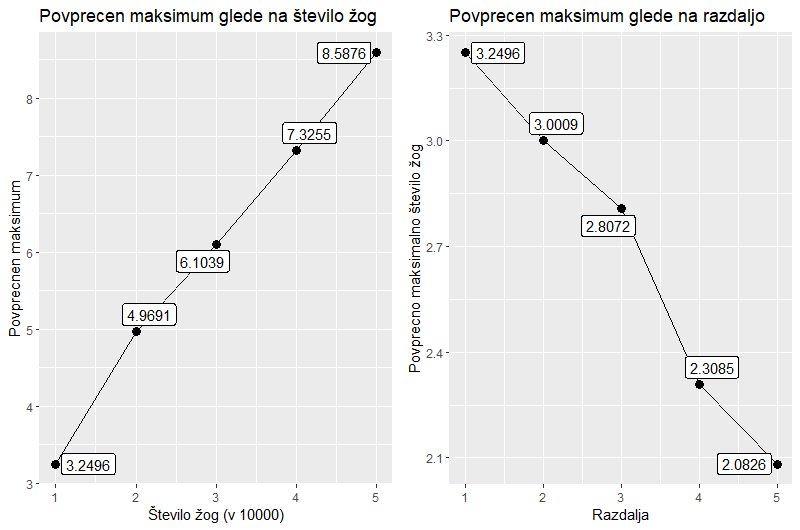
\includegraphics[width=12cm, height=6cm]{povprecje_1dim1.png}

Na prvem grafu je prikazano spreminjanje povprečnega maksimalnega števila žog v košu v odvisnosti od števila žog oz. razdalje.
Iz levega grafa je razvidno, da povprečna maksimalna vrednost raste s številom žog, skok pa je največji pri prvem prehodu.
Na podlagi desnega grafa predvidevava, da bo povprečna maksimalna vrednost, pri nespremenjenem številu košev in žog, z večanjem razdalje padala, pri čemer se bo za velike $n$ bližala vrednosti $1$.
\bigbreak


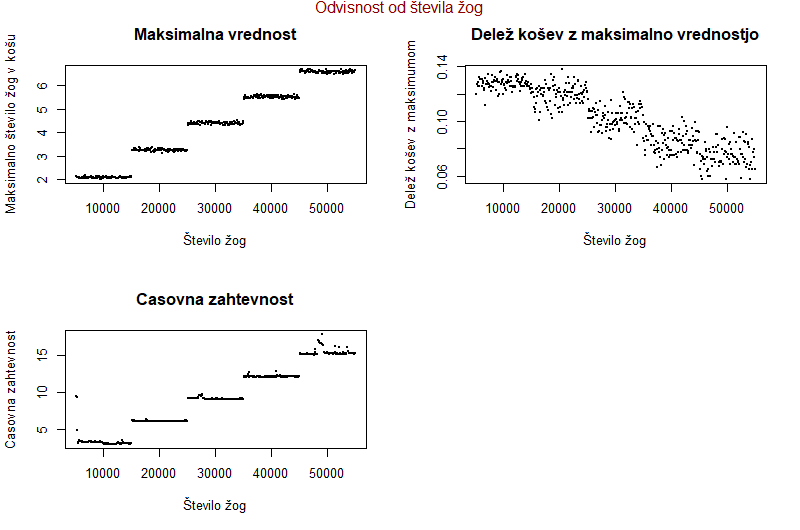
\includegraphics[width=12cm, height=8cm]{dim1_glede_na_stevilo_zog1.png}

Zgornji graf prikazuje razpršenost in gibanje rezultatov glede na število žog. Vsaka pikica predstavlja povprečje opazovane vrednosti pridobljeno s $100$-kratno ponovitvijo poskusa (prej omenjen postopek generiranja rezultatov).
Razvidno je, da za nobeno izbrano količino žog povprečna maksimalna vrednost pretirano ne odstopa. Večje razlike so opazne pri deležu košar z maksimalno vrednostjo. Na podlagi grafa predvidevava, da z naraščanjem števila žog pada delež košev z maksimalno vrednostjo,
hkrati pa so rezultati vedno bolj razpršeni (imajo večji odklon).
Časovna zahtevnost dokaj enakomerno narašča, na vsakih novih 10000 žog se poveča za približno 2,4 sekunde, pri tem pa se razpršenost le minimalno spreminja.
\bigbreak


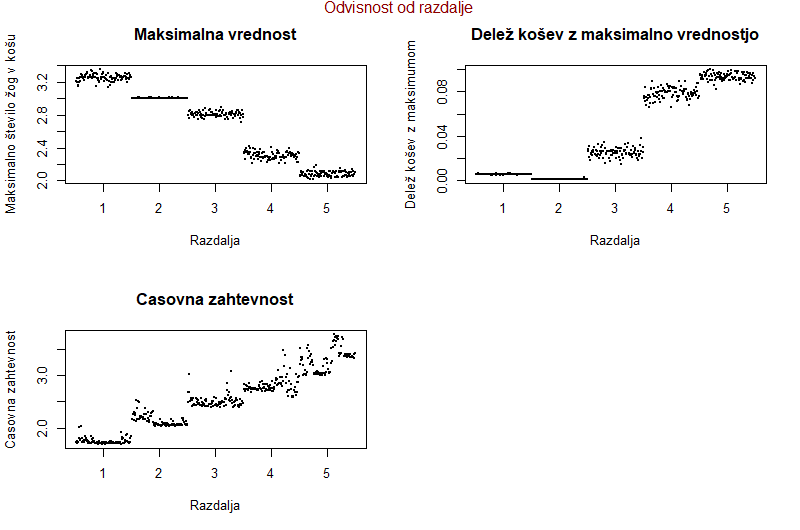
\includegraphics[width=12cm, height= 8cm]{dim1_glede_na_razdaljo1.png}

Druga sprmenljivka, ki naju je zanima je razdalja oz. število sosedov, njen vpliv pa je prikazan na zgornjem grafu.
Tokrat opazimo, da se razpršenost deleža košev večaja pri večjih razdaljah. Predvidevava, da z večanjem števila sosedov raste delež košev z maksimalno vrendostjo, saj se žoge pri večjem številu kandidatov razporejajo bolj enakomerno.
Časovna zahtevnost je veliko bolj razpršena, odstopanja se pojavljajo, ker z večanjem sosedov posledično vplivamo na večanje variabilnosti možnih kandidatov z minimalno vrednostjo žog v košari. Ob spreminjanju števila kandidatov pa se nato spreminja časovna zahtevnost.
\bigbreak

\subsubsection{Minimalna vrednost}
Odločila sva se tudi za analizo minimalnega števila žog v koših in deleža košev z minimalnim številom žog.
\bigbreak
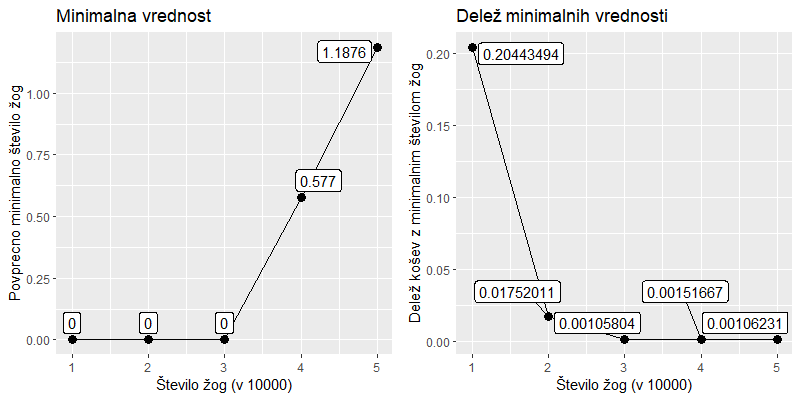
\includegraphics[width=12cm, height=6cm]{minimum.png}

Opazimo, da se z večanjem števila žog minimalna vrednost hitro začne razlikovati od 0, hkrati pa lahko predvidevamo, da se delež košov asimptotsko približuje $0$. 
\bigbreak

\subsection{Dvodimenzionalen problem}
V dvodimenzionalni mreži košev s topologijo torusa sva poskuse izvajala na podoben način, zato sva tudi rezultate za lažjo primerjavo ponazorila podobno.

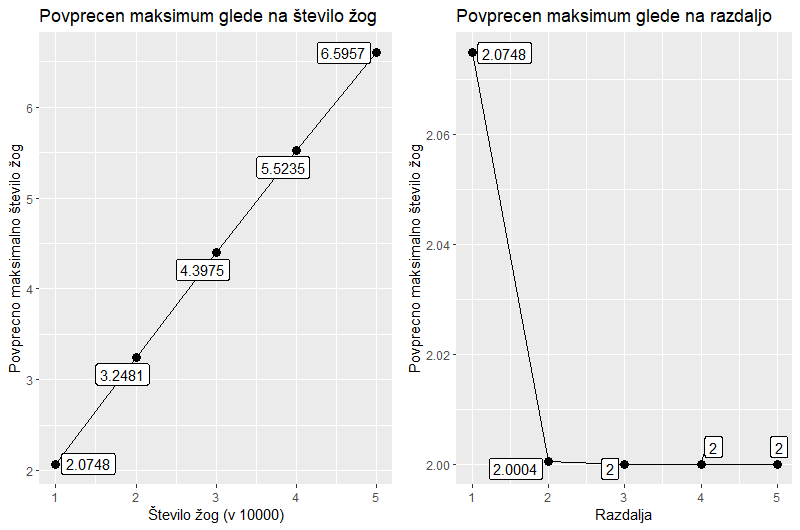
\includegraphics[width=12cm, height=6cm]{povprecje_2dim1.png}

Povprečne maksimalne vrednoti so veliko manjše kot v enodimenzionalnem primeru, saj pride do večje prerazporeditve. Na desnem grafu vrendosti tudi veliko hitreje konvergirajo, kar je pričakovano, saj se število sosedov poveča za faktor $+4$ vsakič ko povečamo razdaljo, 
medtem ko se je v prejšnem primeru povečal le za $+2$.
\bigbreak
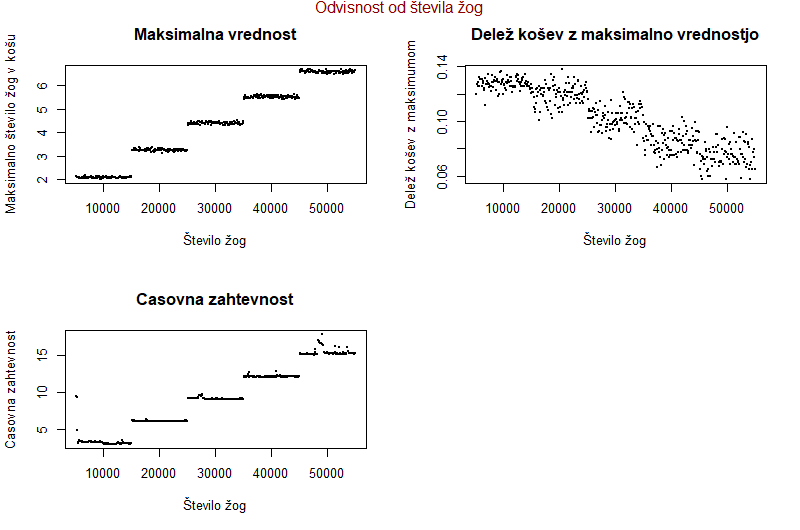
\includegraphics[width=12cm, height= 8cm]{dim2_glede_na_stevilo_zog1.png}

Delež košev z maksimalno vrednostjo je veliko večji kot pri prejšnjem primeru, kar pomeni, 
da se žoge v dvodimenzionalnem modelu razporejajo bolj enakomerno. Vidimo tudi, da 
delež pada z večanjem žog in predvidevava, da se delež premika proti $0$. Časovna zahtevnost je zelo podobna časovni zahtevnosti v eni dimenziji.

\bigbreak
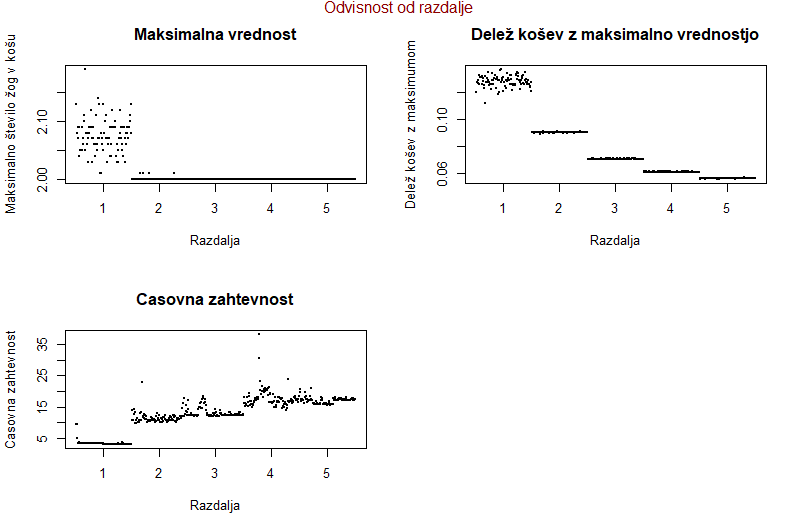
\includegraphics[width=12cm, height= 8cm]{dim2_glede_na_razdaljo1.png}


Takoj opazimo, da se rezultati na razdalji $1$ na vseh treh grafih močno razlikujejo od ostalih. Delež od razdalje $2$ dalje ni več razpršen, torej se rezultati dokaj ustalijo (vsakič dobimo zelo podobne vrednosti). Predvidevava, da bi delež
z večanjem razdalje padal proti 0.
Pri časovni zahtevnosti lahko razpršenost utemeljimo s podobnim argumentom kot v enodimenzionalnem primeru.

\subsection{Tridimenzionalen problem}

Lotila sva se tudi problema soseske, kjer so košare predstavljene v tridimenzionalnem formatu.
V tem primeru sta $b_{i,j,k} $ in $ b_{i',j',l'}$ soseda, ko velja $|i-i'|+|j-j'|+|l-l'| = 1$, ter so sosedje 
$b_{1,j,k} $ in $b_{n,j,k}$, $b_{i,1,k} $ in $b_{i,n,k}$ ter $b_{i,j,1} $ in $b_{i,j,n}$ za $i, j, k \in [n]$.
\\
\\
Generirala sva $100$ povprečij $100$ naključnih poskusov, kjer imamo $k \cdot 8000$ žog in $8000$ košar, $k=1,2, \dots, 5$. 
V spodnjih grafih so prikazana povprečja posameznih rezultatov. 
\bigbreak
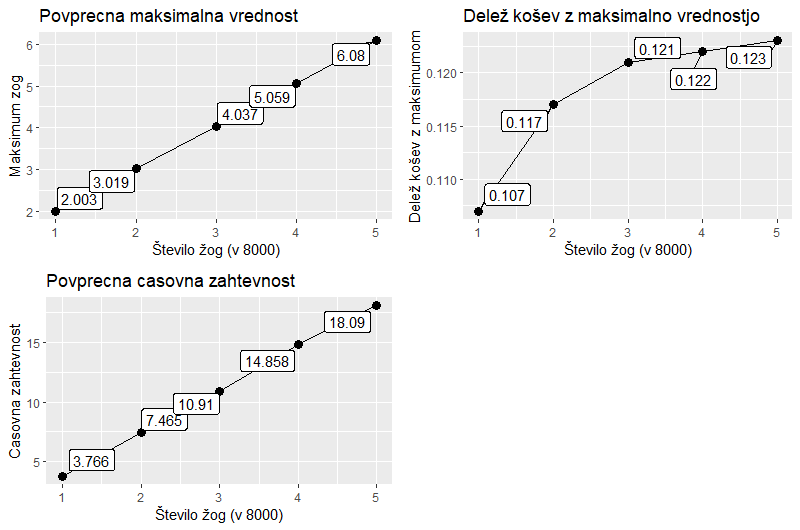
\includegraphics[scale=0.65]{povprecje_3d.png}
\\
Glede na generirane podatke ocenjujeva, da se maksimalna vrednost žog v posamezni košari veča za približno $1,02$ z večanjem
števila žog. Delež košov z maksimalno vrednostjo ima v prvem koraku malo večji skok, kjer se delež poveča za 
$0.01$, potem pa se rast precej umiri, kjer so razlike med koraki približno $0.001$. Časovna zahtevnost se z vsakim večanjem žog poveča za približno $3$ do $4$ sekunde.


\end{document}